\question{Механический смысл вихря и циркуляции.}

\begin{theorem}\label{rotor-m-sense}
  О механическом смысле ротора (вихря)

  Ротор равен отношению циркуляции к площадке, т.е. работе силы вдоль бесконечно
  малого контура.
\end{theorem}
\begin{proof}
  Рассмотрим равенство в т. Стокса (\ref{ST}):

  \begin{align*}
    \iint_{S} \rot \vec{F} \dd \vec{\sigma}
    = \oint_{L^{+}} \vec{F} \dd  \vec{l}
    \eqby{def} \circulation
  \end{align*}

  Выделим в пространстве, где действует \(\vec{F}\), поверхность \(S\),
  окруженную контуром \(L\). К двойному интегралу в левой части равенства
  применима т. Лагранжа о среднем:

  \begin{align*}
    \exists M \in S \colon
      \iint_{S} \rot \vec{F} \dd \vec{\sigma} = \rot \vec{F}(M) \cdot S
  \end{align*}

  Будем стягивать выделенную ранее поверхность в точку \(M_{0}\), получим

  \begin{align*}
    \lim_{\substack{M \to M_{0} \\ S \to 0}}
      \rot \vec{F}(M) \cdot S
    =
    \lim_{\substack{M \to M_{0} \\ S \to 0}}
      \circulation
    \hspace{20pt} \mid \colon S
    \\
    \rot \vec{F}(M_{0}) = \frac{\circulation}{S}
  \end{align*}
\end{proof}

\begin{theorem}
  О механическом смысле циркуляции

  Циркуляция это работа поля по вращению бесконечно малого колеса.
\end{theorem}

\begin{twocolumns}
  \begin{figure}[H]
  \centering

  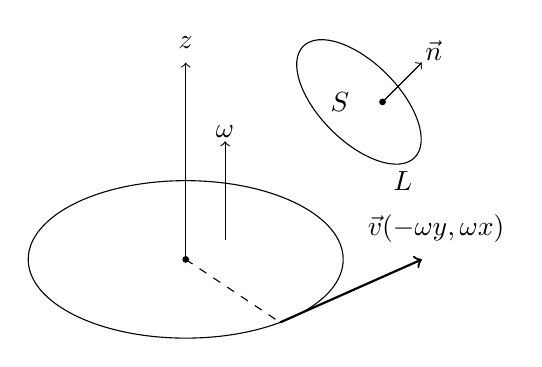
\begin{tikzpicture}
    \coordinate (P) at (1.2, -0.8);
    \draw (0, 0) ellipse (2 and 1);
    \draw[fill = black] (0, 0) circle (1pt);
    \draw[->] (0, 0) -- (0, 2.5) node[pos = 1.1] {\(z\)};
    \draw[->] (0.5, 0.25) -- (0.5, 1.5) node[pos = 1.1] {\(\omega\)};

    \draw[dashed] (0, 0) -- (P);
    \draw[thick, ->] (P) -- (3, 0)
      node[above, pos = 1.1] {\(\vec{v} (-\omega y, \omega x)\)};

    \draw[rotate around = { 135 : (2.2, 2) }]
      (2.2, 2) ellipse (1 and 0.5);
    \draw node[left] at (2.2, 2) {\(S\)};
    \draw node[left] at (3, 1) {\(L\)};

    \draw[fill = black] (2.5, 2) circle (1pt);
    \draw[->] (2.5, 2) -- (3, 2.5)
      node[pos = 1.3] {\(\vec{n}\)};
  \end{tikzpicture}
\end{figure}

  \columnbreak

  Рассмотрим поле линейных скоростей плоско вращающегося тела

  \begin{align*}
    \vec{v}= \under{-\omega y}{P} \vec{i} + \under{\omega x}{Q} \vec{j}
  \end{align*}

  где \(\omega = const\)~--- угловая скорость, которая перпендикулярна
  плоскости вращения.
\end{twocolumns}

\begin{proof}
  Рассмотрим плоскую площадку \(S\), расположенную под углом \(\gamma\) к
  \(Oz\) и ограниченную контуром \(L\). Найдем циркуляцию по этому контуру:

  \begin{align*}
    \circulation_{L}
    = \oint_{L^{+}} P \dd x + Q \dd y
    \eqby{\ref{Green}}
    \iint_{D_{xy}} \left(
      \frac{\partial Q}{\partial x} - \frac{\partial P}{\partial y}
    \right) \dd x \dd y
    \\
    \circulation_{L}
    = \oint_{L^{+}} -\omega y \dd x + \omega x \dd y
    \eqby{\ref{Green}}
    \iint_{D_{xy}} 2 \omega \dd x \dd y
  \end{align*}

  Т.к. \(D_{xy}\) это проекция \(S\) на плоскость \(Oxy\), то
  \(\dd x \dd y = \cos \gamma \dd \sigma\) (пусть \(\cos \gamma > 0\)). Получаем

  \begin{align*}
    \circulation_{L}
    = \iint_{D_{xy}} 2 \omega \dd x \dd y
    = \iint_{S} 2 \omega \cos \gamma \dd \sigma
    = 2 \omega_{n} \iint_{S} \dd \sigma
    = 2 \omega_{n} S_{\text{площадь}}
  \end{align*}

  Где \(\omega_{n}\) это проекция угловой скорости на нормаль к поверхности
  \(S\).
\end{proof}
\begin{corollary}
  Таким образом, если \(\vec{n}_{S} \perp \vec{\omega}\), то работа равна нулю.

  При этом, если учесть механический смысл ротора (\ref{rotor-m-sense}), то

  \begin{align*}
    \rot \vec{F} (M_{0})
    = \frac{\circulation}{S}
    = 2 \omega_{n}
  \end{align*}
\end{corollary}

